\documentclass[10pt]{article}
% 基础格式
\usepackage[UTF8, heading=true]{ctex}          % 中文宏包
% 中文支持（XeLaTeX 编译）
\usepackage{xeCJK}
\usepackage{fontspec}

% 页面设置
\usepackage[
    a4paper,
    left=1.6cm,
    right=1.6cm,
    top=0.9cm,
    bottom=0.8cm
]{geometry}

% 图片排版
\usepackage{graphicx}   % 插入图片的宏包
\usepackage{subfigure}  % 子图片
\usepackage{float}      % 图片固定位置H

\usepackage{enumitem}

% subfig配置
\subfigtopskip=5pt      % 设置子图与上文的距离
\subfigbottomskip=2pt   % 设置不同行子图的间距
\subfigcapskip=0pt      % 设置子图与子标题之间的距离

% 代码块
\usepackage{xcolor}    % 代码颜色
\usepackage{listings}  % 代码块

% 代码格式设置
\lstset{
    language = C++,                                      % 设置语言
    columns = fixed,                                     % 字母间距
    basicstyle = \linespread{0.8} \ttfamily,             % 设置行距，字体
    numbers = none,                                      % 在左侧显示行号
    numberstyle = \footnotesize \color{darkgray},        % 行号格式  
    keywordstyle = \bfseries\color{blue},                % 设定关键字颜色  
    commentstyle = \color[RGB]{0,96,96},                 % 设置代码注释的格式
    stringstyle = \color[RGB]{128,0,0},                  % 设置字符串格式        
    frame = lines,                                        % 左侧显示双竖线
    showstringspaces = false,                            % 不显示字符串中的空格
    breaklines = true,                                   % 自动换行
}

% 页码
\usepackage{lastpage}
\usepackage{fancyhdr}
\pagestyle{fancy}
% 清空默认页眉页脚
\fancyhf{}
% 去掉页眉横线
\renewcommand{\headrulewidth}{0pt}
% 去掉页脚横线
\renewcommand{\footrulewidth}{0pt}
% 右下角页码
\setlength{\footskip}{0pt}
\fancyfoot[R]{
    共 \pageref{LastPage} 页 \quad\quad 第 \thepage 页
}

% 字体设置
\setmainfont{Times New Roman}
\setCJKmainfont{SimSun} % 宋体

\setCJKmainfont[
    AutoFakeBold = true
]{SimSun}

% 华文行楷
\newCJKfontfamily\xingkai{STXingkai}


% 行间距
% 1.5倍行距设置
\renewcommand{\baselinestretch}{1.5}

% 图片引用宏
\newcommand{\fref}[1]{图\ref{#1}}

% 调整标题格式
\ctexset{
    section={
        name = {,、},
        format = {\zihao{4}},
        aftername = \ 
    },
    subsection={
        name = {,、},
        format = {\zihao{-4}},
        aftername = \ 
    },
    subsubsection={
        name = {,、},
        format = {\zihao{-4}},
        aftername = \ 
    }
}

% 正文开始
\begin{document}
\vspace{-0.8cm}

% 左上角标题
\noindent{\xingkai\fontsize{22pt}{22pt}\selectfont 中国科学院大学}

\vspace{1cm}

% 中间标题

\hspace{1cm}\textbf{\songti\zihao{4}试题专用纸}
\vspace{-1.5cm}

% 右上角课程信息
\begin{flushright}
\begin{tabular}{l}
课程编号：180086081201P3001H \\
课程名称：智能计算系统 \\
任课教师：陈云霁、李玲、李威
\end{tabular}
\end{flushright}

\noindent
\makebox[\textwidth]{\leaders\hbox{—}\hfill}

\noindent
{\songti\zihao{-4}
姓名\underline{\hspace{1cm}王峤宇\hspace{1cm}}
\hfill
学号\underline{\hspace{1cm}202518001027021\hspace{1cm}}
\hfill
成绩\underline{\hspace{4cm}}
}

\vspace{0.5cm}
% 正文内容
\begin{center}
    \zihao{-3} 第六七章实验 \quad 深度学习处理器运算器设计实验
\end{center}

% 实验内容、实验步骤、遇到的问题，如何解决、反思思考等内容。
\zihao{-4}

\section{实验内容}

\subsection{实验目的}
掌握深度学习处理器中矩阵运算器的设计原理，能够使用 Verilog 语言实现内积运算
器、矩阵乘向量运算器、矩阵乘法运算器的设计并进行功能仿真。具体包括以下内容：

(1) 理解深度学习处理器加速深度学习运算的原理，理解本实验和深度学习处理器基本模块间的关系。

(2) 使用 Verilog 语言实现内积运算器，理解内积运算器的基本结构，掌握基础的硬件设计流程，完成模块inner\_product\_4x16.v的功能仿真。

(3) 在内积运算器的基础上，使用 Verilog 语言实现矩阵乘向量运算器，加深对深度学习处理器加速原理的理解，补全模块matrix\_vector\_mult\_4x4x16.v的verilog代码，并完成功能仿真。

(4) 在内积运算器、矩阵乘向量运算器的基础上，使用 Verilog 语言实现矩阵乘法运算器，加深对矩阵运算单元的理解，补全模块matrix\_mult\_4x4x4x16.v的verilog代码，并完成功能仿真。

\subsection{设计原理}

\subsubsection{内积运算器设计原理}
提供的已经设计好的内积运算器是一个简易的设计，没有考虑时序性能以及资源开销。内积运算做的是两个向量之间逐元素相乘后求和的运算，输入是两个长度为16的向量，输出是一个数。对应module的port为两个4元素的16bit浮点数向量，和32bit的输出结果。乘法运算和加法运算直接使用了Verilog的乘法和加法运算符实现，指定数据类型为16bit符号数整型数据。

相比实验指导书提供的内积运算器框架示意图，inner\_product\_4x16.v的时序逻辑部分，只对输入数据打了一拍，然后直接输出内积运算结果，没有对输出数据进行打拍。

\subsubsection{矩阵乘向量运算器设计原理}
矩阵乘向量运算是深度学习中常见的操作，是由内积运算组合而成，由于是矩阵在前，相当于使用向量（列向量）对矩阵每一个行向量求内积结果，得到一个新的向量（列向量），是向量在矩阵（对应神经网络的参数）组成空间中的线性变换。

综上，矩阵乘向量运算器的设计可以直接转化成多个内积运算器，每个内积运算器对应矩阵的一行和输入向量的内积运算，得到输出向量的一个元素。对于4x4的矩阵乘以4x1的向量，输出是4x1的向量，因此需要4个内积运算器。

实验给出的待补全模板代码仅仅是对内积运算器的例化，所以最终的电路中依然是输入数据打一拍之后，直接输出，通过复杂的一拍组合逻辑实现矩阵乘向量运算，基本没有时序性能和资源开销的优化，为最简单的示意代码。

\subsubsection{矩阵乘法运算器设计原理}

通过神经网络计算加深对矩阵乘法的理解，可以将矩阵乘法转化成多个矩阵乘向量运算，这样的话矩阵乘法相当于在做多个向量线性变换的batch运算，所以与矩阵乘向量的设计思路一致，矩阵乘法是多个矩阵乘向量运算的组合，每个矩阵乘向量运算对应矩阵乘法结果中的一个行向量。输入是两个4x4的矩阵，输出是一个4x4的矩阵，因此需要4个矩阵乘向量运算器。

\section{实验步骤及结果}
在理解了三个模块的层级关系之后，完成对应verilog文件的模块例化补全之后进行仿真实验验证。

实验过程中，提供的data文件并不能满足所有的实验要求，需要自己配置实验数据进行验证，但考虑到手动配置的可靠性和效率都比较差，选在在cpp仿真测试文件中直接生成测试用的随机数据。


\subsection{tb\_inner\_product}

三个测试脚本文件的测试逻辑基本一致，首先分析测试流程。

在主要的main函数中，读取数据，初始化模块之后通过while循环测试。在初始化阶段将所有的输入数据置为0，同时给定复位信号；仿真结束条件为60个时间步；在while循环中，首先通过对sim\_time的检测，翻转时钟，产生时钟激励；第5个时间步的时候取消复位信号；在第9个时间步时（此时时钟在低电平）产生对应的输入数据激励，然后保持；在第11个时间步（上升沿前），置位enable开始计算；保持一定时间后采样结果，开始比对结果，最后结束仿真。

在生成测试数据部分，因为需要验证的计算功能并不复杂， 采用直接for循环计算的方式计算随机数据的期望结果，对应的代码如下，通过类型转换严格保证数据位宽的正确性，避免了数据溢出等问题。

\begin{lstlisting}[language=C++]
bool gen_inner_test_data(int len, vector<int16_t>& activation, vector<int16_t>& weight, int32_t& expected_result) {
    mt19937 gen(12345);
    uniform_int_distribution<> dis(0, 65535/16);

    for (int i = 0; i < len; i++) {
        activation.push_back(dis(gen));
        weight.push_back(dis(gen));
    }

    // 计算预期结果
    int64_t sum = 0;
    for (int i = 0; i < len; i++) {
        sum += static_cast<int64_t>(activation[i]) * static_cast<int64_t>(weight[i]);
    }
    expected_result = static_cast<int32_t>(sum & 0xFFFFFFFF); // 模拟32位结果
    return true;
}
\end{lstlisting}

向量内积的仿真结果日志如\fref{fig:res_1}所示，随机生成的数据及host端计算的期望结果与仿真结果完全一致，验证了内积运算器的功能正确性。
\begin{figure}[H]
    \centering
    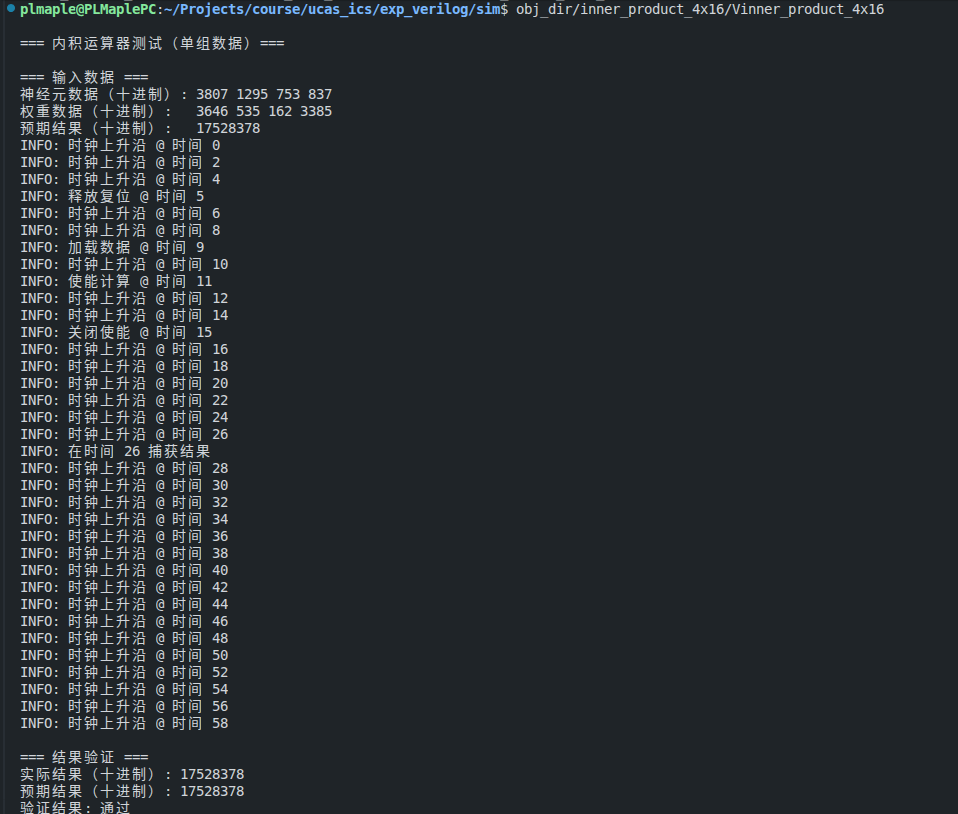
\includegraphics[width=0.7\textwidth]{img/res_1.png}
    \caption{tb\_inner\_product仿真结果日志}
    \label{fig:res_1}
\end{figure}

对应的仿真波形\fref{fig:res_1_wave}所示，数据激励情况与日志输出一致，其中可以看到在enable置位后的下一拍，模块得到计算结果result。
\begin{figure}[H]
    \centering
    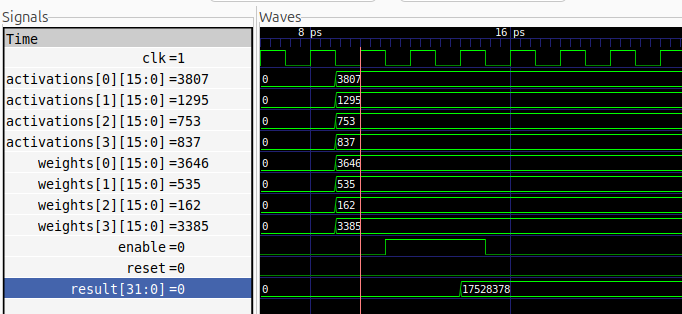
\includegraphics[width=0.8\textwidth]{img/res_1_wave.png}
    \caption{tb\_inner\_product仿真波形}
    \label{fig:res_1_wave}
\end{figure}

\subsection{tb\_matrix\_vector}
矩阵乘向量的随机测试数据生成代码如下:
\begin{lstlisting}[language=C++]
// 生成方阵和向量的测试数据
// 生成方阵和向量的测试数据
bool gen_matrix_vector_test_data(int size, vector<int16_t>& activations, vector<int16_t>& weights, vector<int32_t>& expected_results) {
    
    mt19937 gen(12345);
    uniform_int_distribution<> dis(0, 65535/16);

    for (int i = 0; i < size; i++) {
        activations.push_back(dis(gen));
    }

    // 生成随机数据
    for (int i = 0; i < size * size; i++) {
        weights.push_back(dis(gen));
    }

    // 计算预期结果
    for (int i = 0; i < size; i++) {
        int64_t sum = 0;
        for (int j = 0; j < size; j++) {
            // 矩阵乘向量，每行乘以向量对应元素累加
            sum += static_cast<int64_t>(weights[i*size + j]) * static_cast<int64_t>(activations[j]);
        }
        expected_results.push_back(static_cast<int32_t>(sum & 0xFFFFFFFF)); // 模拟32位结果
    }
    return true;
}
\end{lstlisting}

对应仿真测试脚本的日志输出如\fref{fig:res_2}所示，随机生成的数据及计算的期望结果与仿真结果完全一致，验证通过。
\begin{figure}[H]
    \centering
    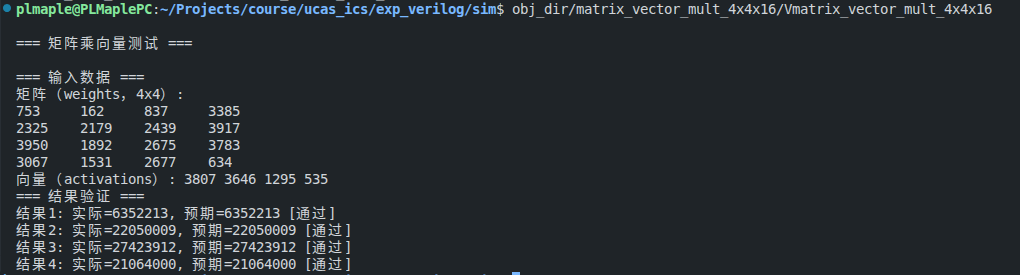
\includegraphics[width=0.8\textwidth]{img/res_2.png}
    \caption{tb\_matrix\_vector仿真结果日志}
    \label{fig:res_2}
\end{figure}

对应的仿真波形如\fref{fig:res_2_wave}所示，数据激励情况与日志输出一致，由于只有例化，模块计算结果没有额外的延迟，但是每一个内积模块都要对输入数据进行打拍，有一定的存储资源冗余，这样的冗余换来的低扇出显然是不合理的。
\begin{figure}[H]
    \centering
    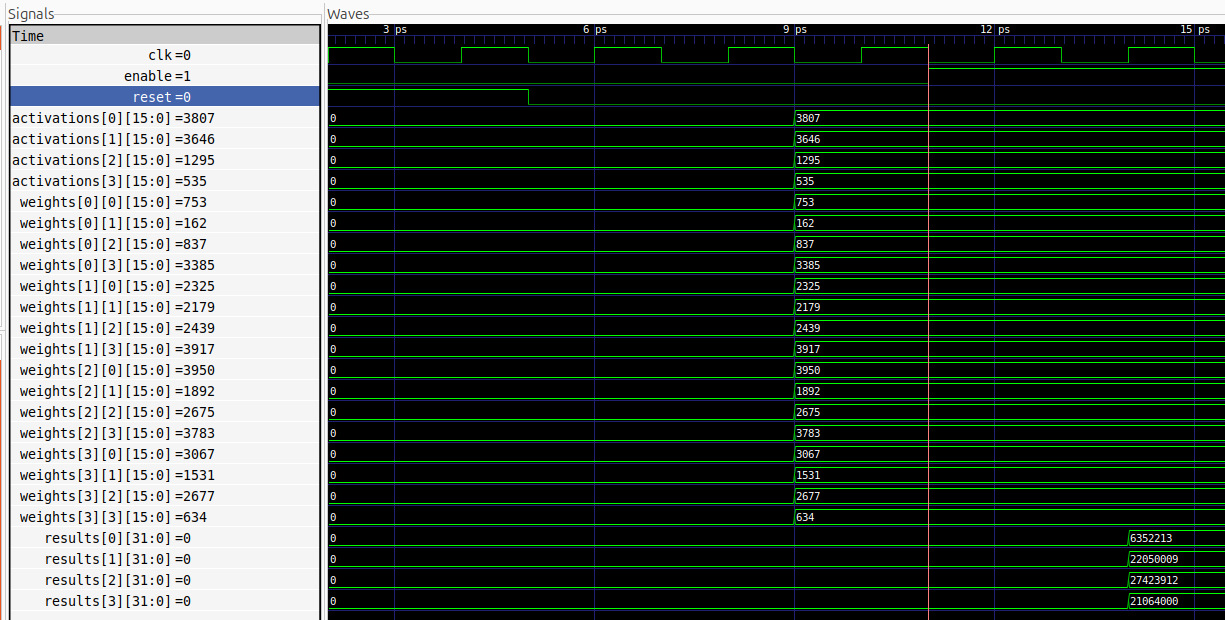
\includegraphics[width=0.8\textwidth]{img/res_2_wave.png}
    \caption{tb\_matrix\_vector仿真波形}
    \label{fig:res_2_wave}
\end{figure}

\subsection{tb\_matrix\_mult}
对应的随机测试数据生成代码如下:
\begin{lstlisting}[language=C++]
bool gen_matrix_test_data(int size, vector<int16_t>& activations, vector<int16_t>& weights, vector<int32_t>& expected_results) {
    
    mt19937 gen(12345);
    uniform_int_distribution<> dis(0, 65535/16);

    for (int i = 0; i < size * size; i++) {
        activations.push_back(dis(gen));
    }

    // 生成随机数据
    for (int i = 0; i < size * size; i++) {
        weights.push_back(dis(gen));
    }

    // 计算预期结果
    // 按activation 行 batch计算
    for (int i = 0; i < size; i++) {
        for (int j = 0; j < size; j++) {
            int32_t sum = 0;
            for (int k = 0; k < size; k++) {
                sum += static_cast<int32_t>(activations[i * size + k]) * weights[j * size + k];
            }
            expected_results.push_back(sum);
        }
    }
    return true;
}
\end{lstlisting}

对应仿真测试脚本的日志输出如\fref{fig:res_3}所示，随机生成的数据及计算的期望结果与仿真结果完全一致，验证通过。
\begin{figure}[H]
    \centering
    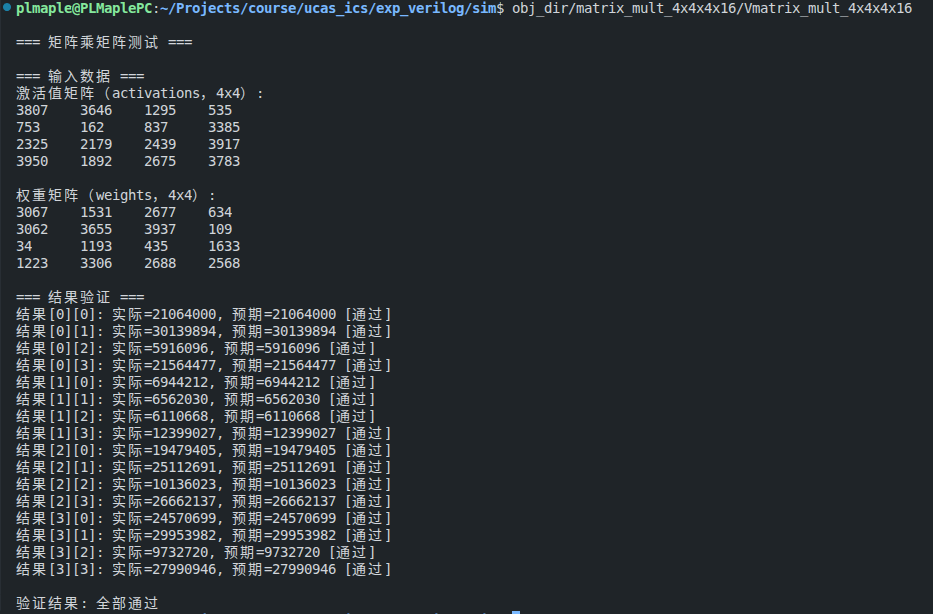
\includegraphics[width=0.8\textwidth]{img/res_3.png}
    \caption{tb\_matrix\_mult仿真结果日志}
    \label{fig:res_3}
\end{figure}

对应的仿真波形如\fref{fig:res_3_wave}所示，以激活值的前两个向量为例进行波形分析，数据激励情况与日志输出一致，由于只有例化，模块计算结果没有额外的延迟，与矩阵乘向量运算器有相同的问题，现在每一个模块都要对输入的weight矩阵进行打拍，存在很高的资源冗余，可以进行适当的优化。

\begin{figure}[H]
    \centering
    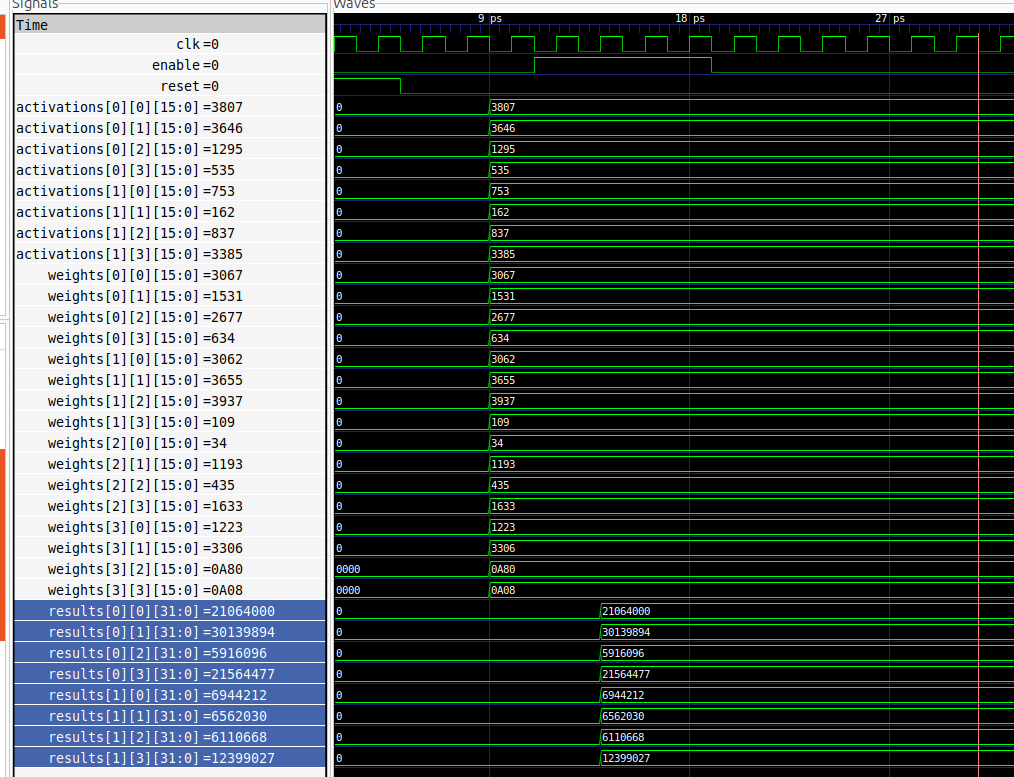
\includegraphics[width=0.8\textwidth]{img/res_3_wave.png}
    \caption{tb\_matrix\_mult仿真波形}
    \label{fig:res_3_wave}
\end{figure}

\section{遇到的问题及解决方法}
\subsection{提供Makefile脚本的相对路径问题}
在使用verilator编译verilog和对应的仿真测试cpp脚本时，对cpp文件的路径指定使用的是相对路径，而在编译的过程中，会切换工作路径到编译文件夹中，所以在编译的过程中会因为找不到.cpp文件而报错，如\fref{fig:error}所示。

\begin{figure}[H]
    \centering
    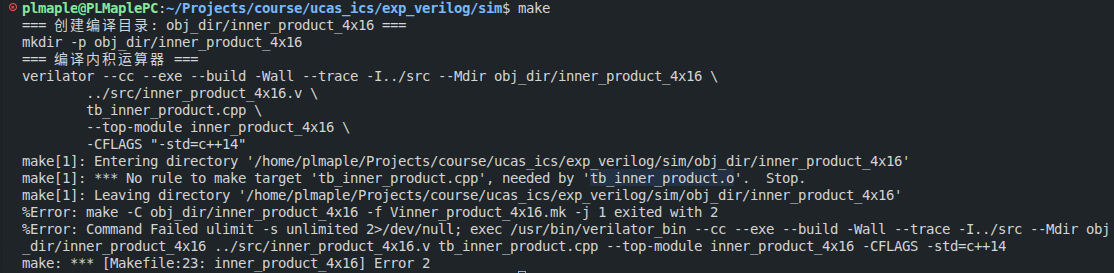
\includegraphics[width=0.8\textwidth]{img/error_1.png}
    \caption{编译错误日志}
    \label{fig:error}
\end{figure}

解决方法是将Makefile中对.cpp文件的路径指定改成绝对路径，最终对Makefile脚本的修改如下，在sim路径下的Makefile中，使用\$(SIM\_DIR)变量指定cpp文件的绝对路径。

\begin{lstlisting}[language=C++]
SIM_DIR = $(CURDIR)
# 内积运算器
inner_product_4x16:
	@echo "=== 创建编译目录: $(OBJ_DIR)/$@ ==="
	mkdir -p $(OBJ_DIR)/$@
	@echo "=== 编译内积运算器 ==="
	$(VERILATOR) $(VERILATOR_FLAGS) --Mdir $(OBJ_DIR)/$@ \
		$(SRC_DIR)/$@.v \
		$(SIM_DIR)/tb_inner_product.cpp \
		--top-module $@ \
		-CFLAGS "$(CXXFLAGS)"
\end{lstlisting}

\section{反思思考}
本次实验提供的代码模板设计过于简单，但很清晰的展示了这三种运算对应底层电路模块之间的关系，也通过神经网络学习和本次模块实现的过程加深了自己对矩阵乘法、向量运算的理解。

此外，针对这样一个简易的代码模板，也可以思考很多的优化方向。首先是结果分析中提到的资源冗余。由于大量的直接例化子模块，每一个子模块都会对输入数据进行打拍存储，导致了大量的资源冗余，实际的设计过程中，完全可以将内积运算的组合逻辑单独抽离出来作为一个模块，然后在矩阵乘向量、矩阵乘法模块中调用时在对输入打拍，这样将输入数据扇出的问题暴露出来，有利于综合器自行判断是否duplicate优化扇出；此外，向量内积模块只是简单的16bit整形数据的乘法运算，实际应用中对大位宽整形、浮点数的乘法运算设计都更加复杂，尤其是浮点数乘法涉及到指数部分的对齐、尾数部分的乘法、结果规格化等复杂的逻辑设计，需要进行流水化设计或者multicycle设计，增加吞吐量。此外，向量内积作为最基础的运算，如果要扩大规模，其reduce sum的操作也有很多的优化空间，比如采用华莱士树等优化结构来提升性能。

\end{document}